
%(BEGIN_QUESTION)
% Copyright 2006, Tony R. Kuphaldt, released under the Creative Commons Attribution License (v 1.0)
% This means you may do almost anything with this work of mine, so long as you give me proper credit

On the job, you are sent to troubleshoot a brand-new control system, consisting of a pneumatic liquid level transmitter connected to a pneumatic controller, which in turn drives a pneumatic control valve.  The process vessel, piping, control valve, controller, and level transmitter are all brand-new: they even sport a fresh coat of paint.

$$\includegraphics[width=15.5cm]{i00140x01.eps}$$

According to the unit operator, this level control system has {\it never} worked.  As she shows you, the liquid level inside the vessel is so low that the level gauge (LG) registers empty, yet the controller is commanding the valve 100\% open, which of course continues to drain the vessel and prevent any liquid level from accumulating.

Being versed in process control theory, you decide to check how the controller is configured.  Looking inside the controller case, you notice the controller is set for {\it direct} action: an increasing PV results in an increasing output signal (MV), which will move the air-to-close valve more toward the ``closed'' state.  

Realizing how to fix the problem, you reach inside the controller and move a lever that switches it into {\it reverse} action mode.

\vskip 10pt

Explain why this fixes the problem.

\vskip 20pt \vbox{\hrule \hbox{\strut \vrule{} {\bf Suggestions for Socratic discussion} \vrule} \hrule}

\begin{itemize}
\item{} Explain the significance of the ``newness'' of this process.  How would your assumptions differ if you saw this process vessel was old and rusted instead of shiny-new?
\item{} How do you suppose the controller got to be mis-configured in the first place?
\item{} What would have to be different in this control system to permit a direct-acting controller instead of a reverse-acting controller?
\item{} Suppose you did not discover the controller's action set for direct action.  If the controller had been left in manual mode instead of automatic mode, could this account for the problems exhibited by this system?
\end{itemize}

\underbar{file i00140}
%(END_QUESTION)





%(BEGIN_ANSWER)


%(END_ANSWER)





%(BEGIN_NOTES)

This was a real problem I encountered on the job, while working at an oil refinery!

\vskip 10pt

A good diagnostic principle to keep in mind when approaching problems is to ask how {\it new} the malfunctioning system is.  Faults in old systems tend to be quite different in nature from faults in brand-new systems.  The fresh coat of paint on the process vessels and piping is a clue to troubleshooting the system: with it being so new, it {\it probably never worked correctly}, and so the fault is most likely some form of mis-configuration.  In this particular case, the problem turned out to be incorrect controller action.  

Faults in old (previously working) systems tend to be related to wear and tear rather than mis-configuration.  Of course, it is always possible for someone to mis-configure an instrument in a system that previously worked for years, but this is unlikely because the problem(s) caused by that mis-configuration often appear immediately and are therefore easily corrected by the perpetrator.

The same rule holds true for mature systems recently rebuilt.  When a process or a machine fails to operate normally after being rebuilt, the responsible fault(s) are most often related to mis-configuration or mis-installation rather than component aging.

\vskip 20pt \vbox{\hrule \hbox{\strut \vrule{} {\bf Virtual Troubleshooting} \vrule} \hrule}

This question is a good candidate for a ``Virtual Troubleshooting'' exercise.  Presenting the diagram to students, you first imagine in your own mind a particular fault in the system.  Then, you present one or more symptoms of that fault (something noticeable by an operator or other user of the system).  Students then propose various diagnostic tests to perform on this system to identify the nature and location of the fault, as though they were technicians trying to troubleshoot the problem.  Your job is to tell them what the result(s) would be for each of the proposed diagnostic tests, documenting those results where all the students can see.

During and after the exercise, it is good to ask students follow-up questions such as:

\begin{itemize}
\item{} What does the result of the last diagnostic test tell you about the fault?
\item{} Suppose the results of the last diagnostic test were different.  What then would that result tell you about the fault?
\item{} Is the last diagnostic test the best one we could do?
\item{} What would be the ideal order of tests, to diagnose the problem in as few steps as possible?
\end{itemize}



\vfil \eject

\noindent
{\bf Prep Quiz:}

{\it Direct action} for a process controller is defined as:

\begin{itemize}
\item{} The process variable (PV) signal increases as the setpoint (SP) signal increases
\vskip 5pt
\item{} The process variable (PV) signal decreases as the setpoint (SP) signal increases
\vskip 5pt
\item{} The output (MV) signal decreases as the process variable (PV) signal increases 
\vskip 5pt
\item{} The output (MV) signal increases as the process variable (PV) signal increases
\vskip 5pt
\item{} The setpoint (SP) signal increases as the process variable (PV) signal increases 
\vskip 5pt
\item{} The setpoint (SP) signal decreases as the process variable (PV) signal increases 
\end{itemize}


\vfil \eject

\noindent
{\bf Prep Quiz:}

{\it Reverse action} for a process controller is defined as:

\begin{itemize}
\item{} The process variable (PV) signal increases as the setpoint (SP) signal decreases
\vskip 5pt
\item{} The process variable (PV) signal decreases as the setpoint (SP) signal decreases
\vskip 5pt
\item{} The output (MV) signal decreases as the process variable (PV) signal increases 
\vskip 5pt
\item{} The output (MV) signal increases as the process variable (PV) signal increases
\vskip 5pt
\item{} The setpoint (SP) signal increases as the process variable (PV) signal increases 
\vskip 5pt
\item{} The setpoint (SP) signal decreases as the process variable (PV) signal increases 
\end{itemize}


%INDEX% Basics, control loop troubleshooting: determining cause of control problem
%INDEX% Process: receiver vessel liquid level control (generic)

%(END_NOTES)


